\documentclass[journal]{IEEEtran}
%\usepackage[left=2.2cm,right=2.2cm,top=2.5cm,bottom=2.5cm]{geometry}
\usepackage[utf8]{inputenc}
\usepackage[english]{babel}
\usepackage{minted}
\usepackage{booktabs}
\usepackage{amsmath}
\usepackage{float}
\usepackage{mathtools}
\usepackage{color}
\usepackage{amsthm}
\usepackage{parskip}
\usepackage{graphicx}
\usepackage{epstopdf}
\usepackage{amssymb}

\theoremstyle{definition}
\newtheorem{defn}{Definition}[section]


\usepackage[binary-units=true]{siunitx}

\newcommand{\py}[1]{\mintinline{python}{#1}}
\newcommand{\java}[1]{\mintinline{java}{#1}}
\newcommand{\sql}[1]{\mintinline{sql}{#1}}

\renewcommand{\epsilon}{\varepsilon}
\renewcommand{\theta}{\vartheta}
\renewcommand{\kappa}{\varkappa}
\renewcommand{\rho}{\varrho}
\renewcommand{\phi}{\varphi}

\usepackage{hyperref}

\title{Architecture and Performance of Computer Systems \\ Project on Client-Server Application Performance}
\author{Gilles Peiffer (24321600), Liliya Semerikova (64811600)}
\date{January 6, 2020}

\begin{document}

\maketitle

\begin{abstract}
	This paper studies the performance of a client-server application (more specifically, a MariaDB server and a remote computer sending randomized SQL queries to that server) in order to first measure the effect of various parameters (such as the query type or the rate at which queries are sent) on the response time of the application, and second, to compare these results to the expected values using the various models of queueing theory.
\end{abstract}

\section*{Introduction}
The answers to the various tasks are given in Sections~\ref{sec:task1} and \ref{sec:task2}.
Section~\ref{sec:char} describes how to reproduce the experiments we did.

\section{Measurements}
\label{sec:task1}
For the first task, we first study the average query response time (and the influence of various parameters on it), then we try to find out what factors influence the response time, and where potential bottlenecks lie.

\subsection{Characteristics for Reproducibility}
\label{sec:char}
All experiments were done on two different physical computers:
\begin{itemize}
	\item The server was MariaDB 10.4.11 running on an Early 2015 MacBook Pro with Ubuntu 18.04 LTS ``Bionic Beaver'', with \SI{8}{\giga\byte} of \SI{1867}{\mega\hertz} of DDR3 RAM memory, a \SI{2.9}{\giga\hertz} Intel Core i5 CPU, an Intel Iris Graphics 6100 \SI{1536}{\mega\byte} GPU and \SI{500}{\giga\byte} of Flash storage.
	\item The remote client was running on a 2016 MacBook Pro with macOS Catalina 10.15.2, with \SI{8}{\giga\byte} of \SI{2133}{\mega\hertz} of LPDDR3 RAM memory, a \SI{2.9}{\giga\hertz} Dual-Core Intel Core i5 CPU, an Intel Iris Graphics 550 \SI{1536}{\mega\byte} GPU and \SI{251}{\giga\byte} of Flash storage.
\end{itemize}

The tests were done on various networks:
\begin{itemize}
	\item a WiFi network in one of the team members' student residence, on which the final tests were done (the ones appearing on plots), and
	\item the home network of the other team member.
\end{itemize}
This network has a download speed of \SI{62}{\mega\bit\per\second} and an upload speed on the order of \SI{6}{\mega\bit\per\second} according to the \href{https://fast.com/en/gb}{\url{FAST.com}} speed test.

For the measurements, no significant warmup was needed, as no amount of queries showed any signs of instability beyond what one would expect on a real-world physical network.
All tests were repeated multiple times, and under different network loads, while final results were obtained when there was no other activity on the network.

Every query is made using a new connection, on a different thread.
For this purpose, we defined a new Java class, \java{SQLThread}, which extends the \java{Thread} class, queries the database when its \java{run()} method is called.
The server is configured to allow up to three concurrent threads, by using the \mintinline[breaklines]{bash}{sudo mysqld --user mysql --innodb-thread-concurrency=3} command, unless specified otherwise.

The measurements were written into csv files by the Java code, which was then read by some short Python scripts which generate the plots using \py{pandas}, \py{seaborn}, and \py{matplotlib}.

\subsection{Average Query Response Time}
\begin{defn}[Response time]
	The \emph{response time} is typically treated as the elapsed time from the moment that a user enters a command or activates a function until the time that the application indicates that the command or function has completed.
\end{defn}

The following section studies the influence of the query type and the query rate on the response time of the application.

\subsubsection{Influence of the Query Type}
For this experiment, various types of queries were considered, based on the ones provided in the client template:
\begin{itemize}
	\item ``\java{GetAverage}'' queries compute the average salary over a certain subset of rows of the table, where the number of rows and the starting row are randomly determined\footnote{In order to simplify the modeling task of Section~\ref{sec:task2}, this random value is generated in a way that the number of rows over which the query operates is exponentially distributed.} outside of the timed section and are passed to the server using the \sql{LIMIT} and \sql{OFFSET} keywords.
	\item ``\java{Select}'' queries select a subset of rows (randomly, according to the same rules as for the previous query) and returns the result.
	\item ``\java{Write}'' queries insert a row into the database.
\end{itemize}

For every type, tests were run multiple times, in order to get an idea of the average response time without inter-arrival pauses.
For the actual tests, every thread waits a certain amount of time before starting its execution.
This amount is an exponentially distributed random variable, in order to mimic a Poisson process, where the parameter \(\lambda\) is different for every type of query and depends on the average response time as well as the number of concurrent threads allowed on the MariaDB server.
In order to single out the influence of the query type, this value was chosen so as to make it very improbable that queries would have to wait before being answered (that is, the server had a very low utilization; approximately \(0.03\)).

The result is shown on Figure~\ref{fig:query_influence}.
This figure also contains theoretical results, which are explained in further detail in Section~\ref{sec:task2}.
\begin{figure}[!hbtp]
	\centering
	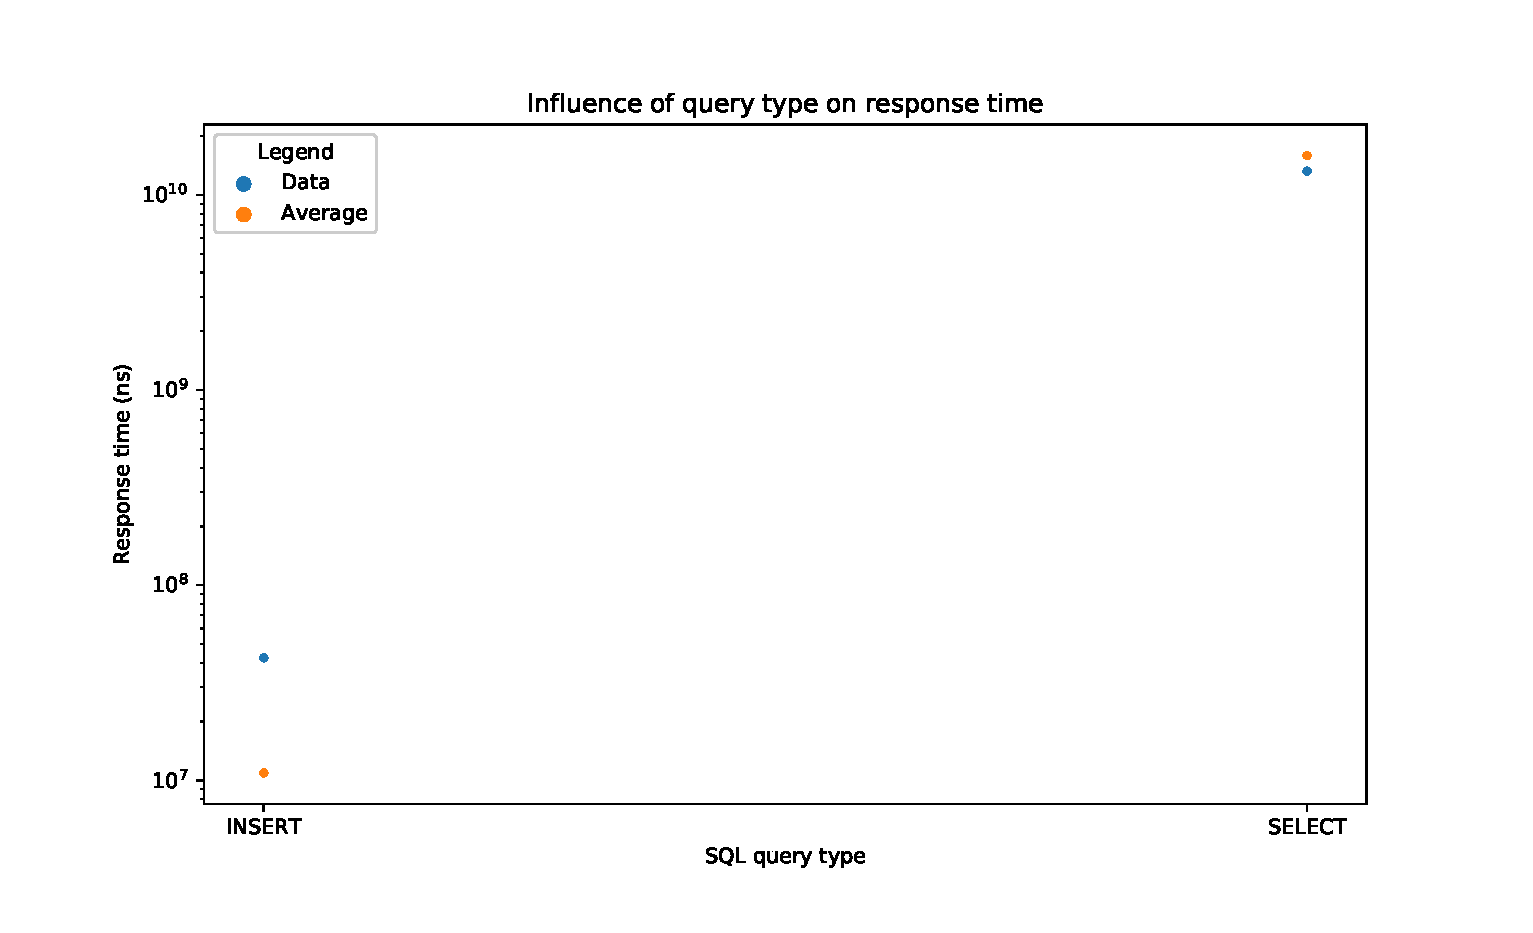
\includegraphics[width=\columnwidth]{../plotting/query_influence}
	\caption{Influence of query type on response time}
	\label{fig:query_influence}
\end{figure}
The \(y\)-axis is shown with logarithmic units in order to clearly show the difference in response time for the various queries.
The \java{Write} query is on average the fastest, which is logical since it only needs to insert a single row into the database; the \java{Select} and \java{GetAverage} queries are separated because the \sql{LIMIT} values are quite different for both requests, with the former having a higher limit than the latter.

\subsubsection{Influence of the Number of Queries Per Second}
Next, in order to control the influence of the rate at which queries are sent, we modify the sleep delay before each thread sends its query.

We still use the same kind of delay as in the previous section, that is, one with exponentially distributed inter-arrival times.
By changing the parameter of the distribution in order to shorten or lengthen the expected waiting time between queries, we were able to observe the influence of the arrival rate on the average response time.

The results of this experiment are shown in Figures~\ref{fig:rate_influence_average} through~\ref{fig:rate_influence_write}.
Again, theoretical results are described in Section~\ref{sec:task2}.
\begin{figure}[!hbtp]
	\centering
	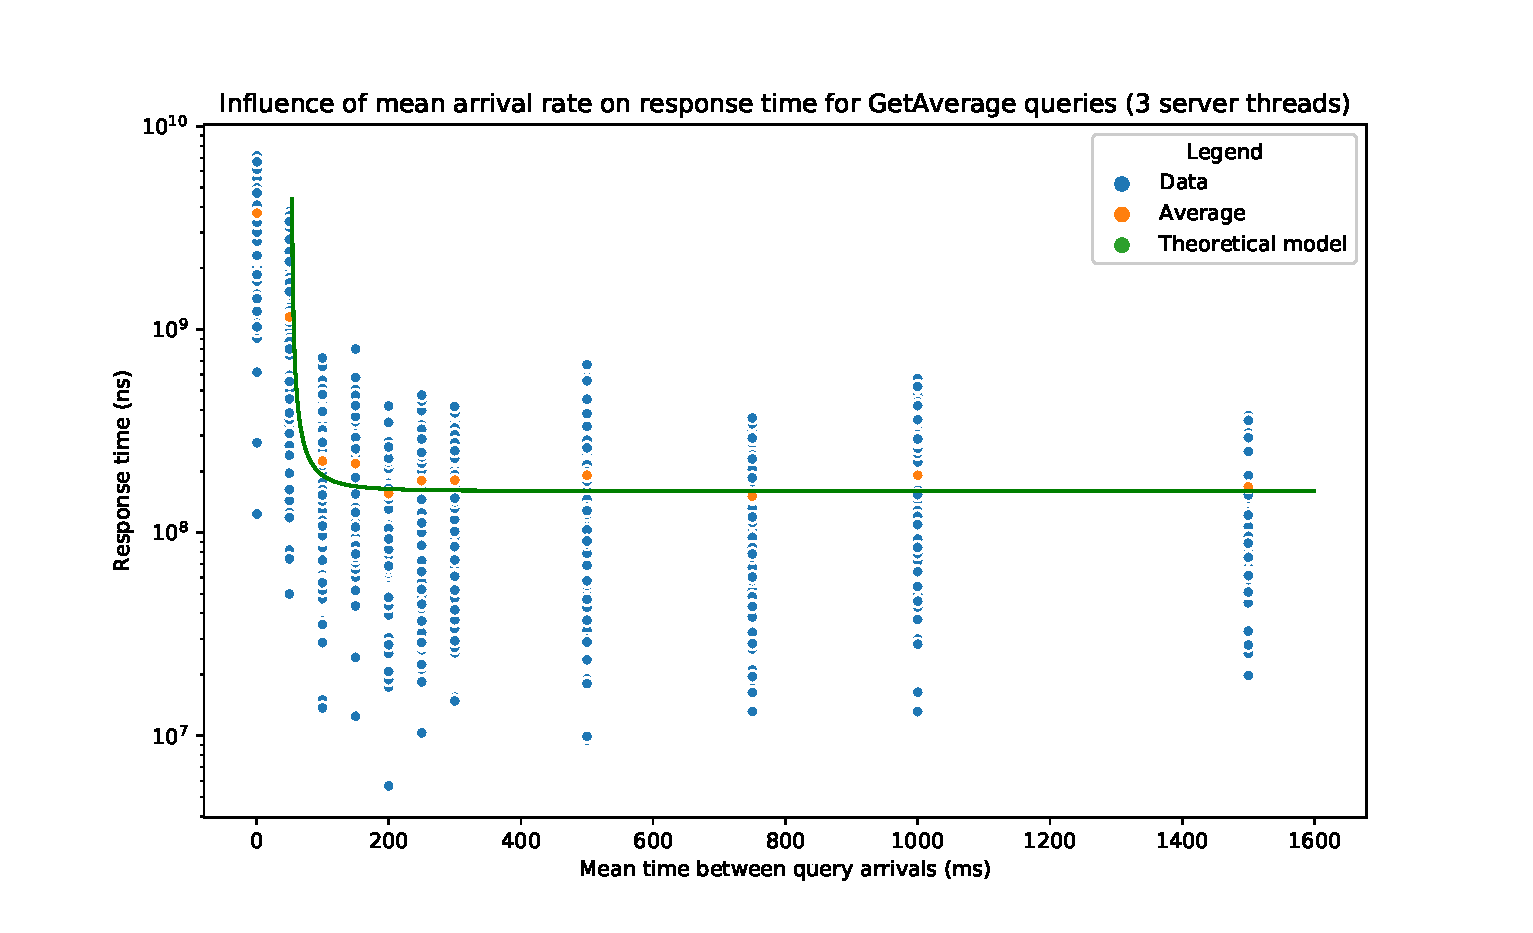
\includegraphics[width=\columnwidth]{../plotting/rate_influence_average}
	\caption{Influence of request rate on response time for the \java{GetAverage} query}
	\label{fig:rate_influence_average}
\end{figure}
\begin{figure}[!hbtp]
	\centering
	\includegraphics[width=\columnwidth]{../plotting/rate_influence_select}
	\caption{Influence of request rate on response time for the \java{Select} query}
	\label{fig:rate_influence_select}
\end{figure}
\begin{figure}[!hbtp]
	\centering
	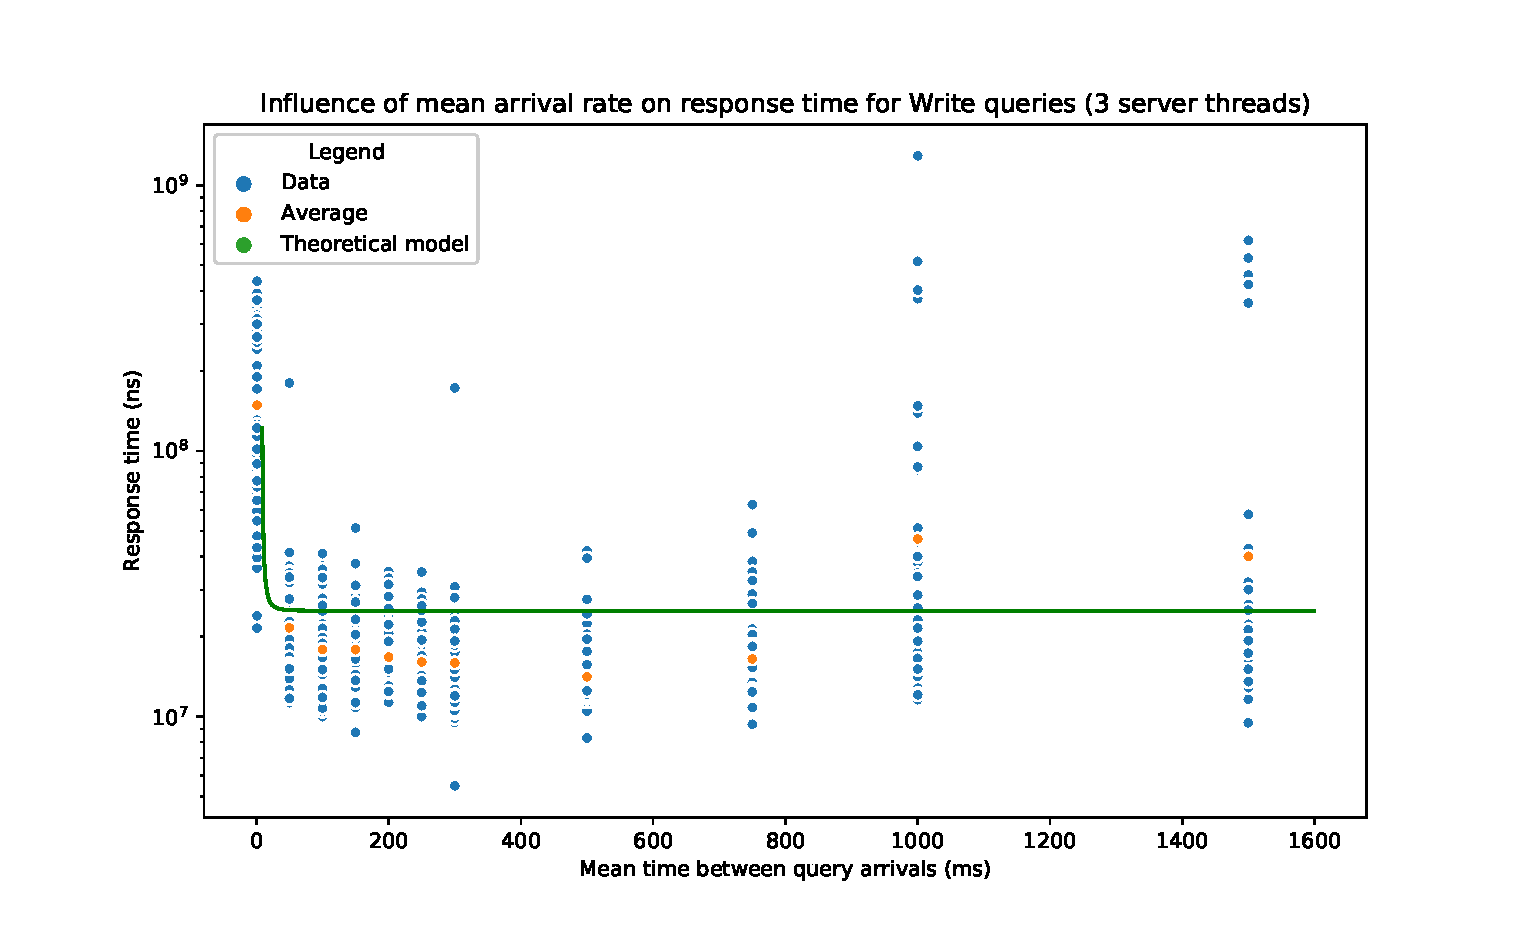
\includegraphics[width=\columnwidth]{../plotting/rate_influence_write}
	\caption{Influence of request rate on response time for the \java{Write} query}
	\label{fig:rate_influence_write}
\end{figure}

As seen on the figures, the larger the mean-interarrival time, the shorter the response time, generally.
This can be explained by the fact that if queries are sent in rapid succession, the model is going to be temporarily saturated, leading to longer waiting times for the queries that arrive later.
On the other hand, if queries are sent with sufficiently large intervals of time between them, then the server will almost be guaranteed to be able to accept a new query as it arrives, meaning that the waiting time is negligible.
This observation is used in Section~\ref{sec:task2} to estimate the service time of the various requests.

\subsection{Factors Influencing the Query Response Time and Possible Bottlenecks}
We have already noted in the previous sections that the query type and the rate at which queries are sent have an influence on the response time.
In this section, we will give some other factors influencing the response time, and identify where bottlenecks lie.

Using the command line tools \mintinline{bash}{top}, \mintinline{bash}{pidstat}, and \mintinline{bash}{nethogs}, we were able to note that the \mintinline{bash}{mysql} process only took up about \SI{2}{\percent} of the total available RAM, whereas CPU usage was usually around \SI{10}{\percent}, though it was slightly higher for the \sql{SELECT}-based queries than for the \sql{INSERT}-based ones (up to \SI{40}{\percent}).

There were on average around \(40\) minor page faults per second and barely any major page faults.
This leads us to believe that the most important factor is the CPU time, since only \SI{10}{\percent} of it was available to the process most of the time, as well as the minor page faults in the RAM, which can each take several hundreds of microseconds according to \cite{pagefault} (which is critical in time-sensitive applications like this one, especially when these faults happen as regularly as they do).

Considering that the \java{Write} queries have a negligible computation time, one can consider them to be a decent indicator of network latency; taking this into account, the network is another factor that can heavily influence the response time of the (short) queries.

One would also expect the number of threads on the server to have a rather large influence on the response time of the server, but as shown on Figure~\ref{fig:thread_influence}, this is not the case for small values of \(n\).
A reasonable expectation to have is that the optimal number of threads on a real computer is going to be close 
The theoretical prediction however explodes for a small number of threads; the reason for this is explained in Section~\ref{sec:task2}.
\begin{figure}[!hbtp]
	\centering
	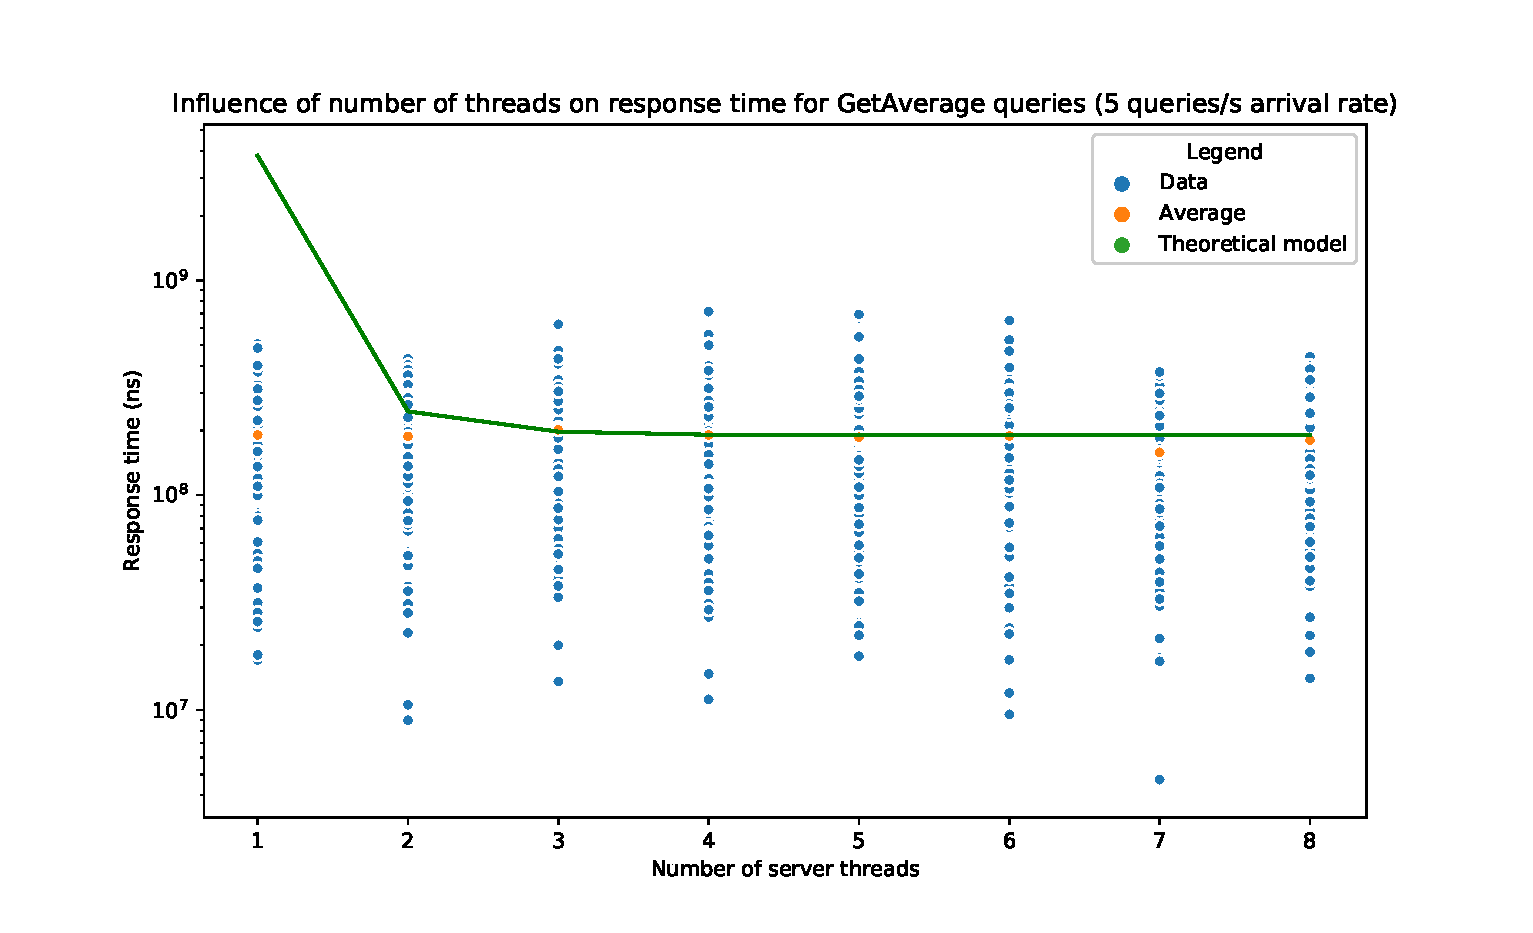
\includegraphics[width=\columnwidth]{../plotting/thread_influence}
	\caption{Influence of the number of server threads on the response time for \java{GetAverage} queries, with an arrival rate \(\lambda = \SI{5}{queries\per\second}\)}
	\label{fig:thread_influence}
\end{figure}

\section{Modeling}
\label{sec:task2}
\subsection{Queueing Station Model}
Using the theoretical results described in the lecture notes, we now attempt to model the client-server application using one of the models from queueing theory covered in class.
Models are described in Kendall notation \cite{kendall}.

As mentioned in the project statement, a choice was made to use Markovian arrivals, i.e., modulated by a Poisson process.
In general, one would expect that using the  \(M \mid G \mid m\) model is the optimal choice from the point of view of its predictive power, given that a database cannot reliably be said to have exponentially distributed service times.
However, the \(M \mid G \mid m\) model is difficult to use due to its complexity (\cite{mgm}), and was not covered as extensively during the lectures\footnote{If one were to really insist, this would require computing the second moment of the service time (a relatively easy task using Python), and then applying the Pollaczek--Khinchine formula: \(\mathbb{E}R = \mathbb{E}S + \frac{\lambda \mathbb{E}S^2}{2(1-\rho)}\), where \(\rho\) is the average number of customers in the service station.}; therefore, we adapted the client code to send requests (for \java{GetAverage} and \java{Select} queries) which have a random parameter (the number of rows on which to operate) that we generate as an exponential random variable.

We make the reasonable assumption that the service time is then a linear function of this number of rows, and hence conclude that it is also exponentially distributed.
This then allows us to satisfy the assumptions needed for the easier, less general \(M \mid M \mid m\) model (\cite{kendall}), for which many theoretical results are readily available.
The final parameter of the model is simply the number of threads; as mentioned in Section~\ref{sec:task1}, \(m=3\) unless specified otherwise.

\subsubsection{Determining the parameters}
In order to model a queueing station with the \(M \mid M \mid 3\) model, one must set an arrival rate \(\lambda\) and a service rate \(\mu\).
As mentioned in the project statement, the service time is equivalent the response time under the assumption that the queuing station is completely empty upon arrival of the query.
One could think to use the very first query response time as a good indicator of this, but to avoid having to deal with increased response times due to cache warmup, we opted for another estimation: the average response time for a very small arrival rate (or equivalently, a very high mean inter-arrival time).
The arrival rate is very easy to obtain, as it is the client program which decides its value.

We then define the \emph{utilization} of the server as
\[
\chi = \frac{\lambda}{m\mu}.
\]
If \(\chi\) is greater than \(1\), then the queue will grow without bound, but if \(\chi < 1\), then the queue is stable and the system has a stationary distribution with probability mass function
\[
\pi_{0} = \left(\sum_{i=0}^{m-1} \frac{a^i}{i!} + \frac{a^m}{m! (1 - \chi)}\right)^{-1},
\]
where \(a = \lambda/\mu\).
One can then compute the expectation of the response time \(R\) as
\begin{equation}
\mathbb{E}R = \frac{1}{\lambda} \left(a + \frac{\chi a^m}{(1 - \chi)^2 m!}\pi_{0}\right).
\end{equation}

However, when analyzing real-life models, one should be wary that these results make several assumptions, the most important one being that the utilization is much smaller than one.

\subsection{Comparison to the Real Data}
It is interesting to compare the model of the previous section to the real-life data that we obtained in Section~\ref{sec:task1}.
As one can observe, the green graphs on the plots are what one would expect from a purely theoretical point of view.
What follows is a discussion of these results.

\begin{itemize}
	\item On Figures~\ref{fig:rate_influence_average} and \ref{fig:rate_influence_select}, the theoretical predictions line up almost perfectly with the data for larger inter-arrival times.
	This indicates that the model is most likely correct, as well as its parameters.
	For smaller inter-arrival times, the model tends to be off by quite a bit, and for small enough values, it even becomes completely unusable.
	This should not come as a surprise; this is all due to the assumptions of the model, namely the assumption that \(\chi \ll 1\).
	The more this is the case, the better the result (hence, for a very small arrival rate, the theoretical model lines up very well with the real data).
	On the other hand, once the utilization gets nearer to one, the results deteriorate, and if it becomes larger than one, the model loses all its value.
	Formulas for the busy period of the system exist as well (see for example \cite{mmm}), but were not covered in class, and were hence not reproduced in this paper.
	\item On Figure~\ref{fig:rate_influence_write}, the results are slightly worse than on the previous two; this can be explained by the fact that the assumption of exponentially distributed service times might not always be valid for the \java{Write} query type.
	\item Finally, Figure~\ref{fig:thread_influence} shows even better that a high utilization is the bane of stationary analysis, whereas for larger values of \(n\), the prediction is almost eerily accurate.
	This is the only instance where a number of threads different from three was used.
\end{itemize}

\section*{Conclusion}
Servers are an ubiquitous part of the modern world, and it is massively important for the computer scientists of tomorrow to be able to understand how they work, both from a practical and theoretical point of view.

On one hand, there are many useful tools which can help with the former, and on the other, there is a whole field of mathematics devoted to modeling and predicting the behaviour of these servers.

\begin{thebibliography}{9}
	\bibitem{pagefault}
	William Cohen, Examining Huge Pages or Transparent Huge Pages performance Red Hat Developer, \href{https://developers.redhat.com/blog/2014/03/10/examining-huge-pages-or-transparent-huge-pages-performance/}{link}, March 10, 2014.
	
	\bibitem{kendall}
	Kendall, D. G. (1953). ``\href{http://projecteuclid.org/euclid.aoms/1177728975}{Stochastic Processes Occurring in the Theory of Queues and their Analysis by the Method of the Imbedded Markov Chain}''. The Annals of Mathematical Statistics. 24 (3): 338. doi:\href{https://projecteuclid.org/euclid.aoms/1177728975}{10.1214/aoms/1177728975}{}. JSTOR \href{https://www.jstor.org/stable/2236285}{2236285}.
	
	\bibitem{mgm}
	Kingman, J. F. C. (2009). ``The first Erlang century—and the next''. Queueing Systems. 63: 3–4. doi:\href{https://link.springer.com/article/10.1007\%2Fs11134-009-9147-4}{10.1007/s11134-009-9147-4}.
	
	\bibitem{mmm}
	Omahen, K.; Marathe, V. (1978). ``\href{https://docs.lib.purdue.edu/cgi/viewcontent.cgi?article=1110\&context=cstech}{Analysis and Applications of the Delay Cycle for the M/M/c Queueing System}''. Journal of the ACM. 25 (2): 283. doi:\href{https://dl.acm.org/doi/10.1145/322063.322072}{10.1145/322063.322072}.
\end{thebibliography}
 
\end{document}
